
%(BEGIN_QUESTION)
% Copyright 2011, Tony R. Kuphaldt, released under the Creative Commons Attribution License (v 1.0)
% This means you may do almost anything with this work of mine, so long as you give me proper credit

In this process, a single ``shutdown controller'' device sends actuating signals to two block valves, actuating them simultaneously.  The purpose of this system is to provide a very high level of assurance that the process line will be able to flow freely and allow production (i.e. high ``security''), at the expense of a lesser dependability (i.e. either block valve failing in the open position would make it impossible to shut down the flow):

$$\includegraphics[width=15.5cm]{i03791x01.eps}$$

The figure given for each block valve in the above diagram is the {\it probability of failure on demand} (PFD) for that valve: the probability that each valve will fail to shut when it is called to shut by the controller.  

\vskip 10pt

Calculate the probability of this block valve system failing to shut off flow in the line, given the probability of each valve to become stuck open (and not close).  This result you calculate will be the PFD for the entire block valve system.

\vskip 10pt

Next, calculate the {\it dependability} of the entire system: the probability that it {\it will} shut off the line when called to do so.

\vskip 20pt \vbox{\hrule \hbox{\strut \vrule{} {\bf Suggestions for Socratic discussion} \vrule} \hrule}

\begin{itemize}
\item{} A very helpful problem-solving technique when working with probabilities is to {\it sketch a logic function diagram} with each line in that diagram labeled with an easy-to-understand description of its real-life meaning.  Sketch such a diagram for this problem, and then explain how that diagram is helpful.
\end{itemize}

\underbar{file i03791}
%(END_QUESTION)





%(BEGIN_ANSWER)

Probability calculate shown using logic symbols:

$$\includegraphics[width=15.5cm]{i03791x02.eps}$$

%(END_ANSWER)





%(BEGIN_NOTES)


%INDEX% Mathematics, probability: complementation
%INDEX% Safety, system reliability: probability of failure on demand (PFD)

%(END_NOTES)


